\documentclass[10pt,aspectratio=169]{beamer}

% Theme & Styling
\usetheme{Madrid}
\usecolortheme{whale}

\usepackage{graphicx}
\usepackage{booktabs}
\usepackage{amsmath,amssymb}
\usepackage{listings}
\usepackage{tikz}
\usetikzlibrary{shapes.geometric, arrows.meta, positioning, shadows}

% Custom Color Palette
\definecolor{primaryblue}{RGB}{30, 58, 138}
\definecolor{secondaryblue}{RGB}{37, 99, 235}
\definecolor{accentgreen}{RGB}{22, 163, 74}
\definecolor{accentred}{RGB}{220, 38, 38}
\definecolor{accentorange}{RGB}{234, 88, 12}
\definecolor{accentpurple}{RGB}{126, 34, 206}
\definecolor{codebg}{RGB}{248, 250, 252}
\definecolor{codeborder}{RGB}{203, 213, 225}

\setbeamercolor{palette primary}{bg=primaryblue,fg=white}
\setbeamercolor{title}{bg=primaryblue,fg=white}
\setbeamercolor{frametitle}{bg=primaryblue,fg=white}
\setbeamercolor{structure}{fg=primaryblue}

% Remove navigation symbols
\setbeamertemplate{navigation symbols}{}

% Title & Author Metadata
\title[E-LongRAG: Final Evaluation]{\textbf{Efficient LongRAG (E-LongRAG)}}
\subtitle{Adaptive Context Filtering, Neural Reranking, Hybrid Search \& Robust Multi-Metric Evaluation}
\author[Pranav, Pavan, Sameer]{\textbf{Pranav Vinodh} \and \textbf{Durga Sai Pavan Gangabattula} \and \textbf{Sameer}}
\institute[Course: Large Language Models]{\textbf{Course: Large Language Models (IT 488) --- Final Endsemester Evaluation} \\ Department of Information Technology, National Institute of Technology Karnataka (NITK), Surathkal}
\date[\today]{\today}

\begin{document}

% ---------------------------------------------------------
% Slide 1: Title Slide
% ---------------------------------------------------------
\begin{frame}
    \titlepage
\end{frame}

% ---------------------------------------------------------
% Slide 2: Executive Presentation Roadmap
% ---------------------------------------------------------
\begin{frame}{Executive Presentation Roadmap}
    \begin{columns}[onlytextwidth,T]
        \begin{column}{0.48\textwidth}
            \begin{block}{\textbf{Part 1: Foundations \& Midsem Architecture}}
                \footnotesize
                \begin{itemize}\setlength\itemsep{1.5pt}
                    \item \textbf{Problem Motivation}: Short-Chunk Fragmentation vs. LongRAG Prompt Bloat.
                    \item \textbf{LongRAG Bottlenecks}: $O(N^2)$ TTFT Attention Latency and $94\%$ Distractor Noise.
                    \item \textbf{Midsem Pipeline}: HyDE Expansion, Paragraph Slicing, MiniLM Reranking.
                    \item \textbf{Adaptive Context Filtering}: Dynamic Score Cutoff $\tau(q)$ and Cosine Deduplication $\delta=0.85$.
                    \item \textbf{Midsem Empirical Results}: $94.9\%$ Prompt Compression and $19.7\times$ Pre-fill Speedup.
                \end{itemize}
            \end{block}
        \end{column}
        
        \begin{column}{0.48\textwidth}
            \begin{block}{\textbf{Part 2: New Endsem Innovations \& Novelty}}
                \footnotesize
                \begin{itemize}\setlength\itemsep{1.5pt}
                    \item \textbf{Innovation 1}: Retrieval Sampling Suite \& Diversity Metric $\text{Div}(\mathcal{S})$.
                    \item \textbf{Innovation 2}: Lightweight Embedding \& Hybrid BM25+RRF Search.
                    \item \textbf{Innovation 3}: Positional ``Lost-in-the-Middle'' Stress Testing (10k Tokens).
                    \item \textbf{Innovation 4}: Automated RAGAS Quality Metrics, EM \& Token F1.
                    \item \textbf{Innovation 5}: Cross-Encoder Sizing \& 42-Point Pareto Sensitivity Frontier.
                    \item \textbf{Innovation 6}: Multi-Reader Engine (CPU vs Gemini vs Groq) \& 10-Tab Dashboard.
                    \item \textbf{Individual Contributions}: Dedicated breakdown slides for each member.
                \end{itemize}
            \end{block}
        \end{column}
    \end{columns}
\end{frame}

% =========================================================
% PART 1: WORK COMPLETED TILL MIDSEM
% =========================================================
\section{Part 1: Work Completed Till Midsem}

% ---------------------------------------------------------
% Slide 3: Problem Motivation: The Long-Context RAG Dilemma
% ---------------------------------------------------------
\begin{frame}{Part 1: Problem Motivation --- The Long-Context RAG Dilemma}
    \begin{columns}[onlytextwidth,T]
        \begin{column}{0.48\textwidth}
            \begin{block}{\textbf{Short-Chunk RAG ($100$--$500$ tokens)}}
                \begin{itemize}\setlength\itemsep{3pt}
                    \item Fragments cross-sentence entity relations.
                    \item Fails on multi-hop questions requiring joint reasoning across distinct sections.
                    \item Boundary loss destroys narrative continuity.
                    \item Multi-hop recall drops below $60\%$.
                \end{itemize}
            \end{block}
        \end{column}
        
        \begin{column}{0.48\textwidth}
            \begin{block}{\textbf{Baseline LongRAG ($\approx 4,000$ tokens)}}
                \begin{itemize}\setlength\itemsep{3pt}
                    \item Preserves full multi-document narrative flow.
                    \item \textbf{Severe Prompt Bloat}: Prompts exceed $5,000+$ tokens.
                    \item \textbf{Massive Distractor Noise}: $>90\%$ of retrieved tokens are irrelevant to query $q$.
                    \item \textbf{Cognitive Context Dilution}: Dilutes reader focus.
                \end{itemize}
            \end{block}
        \end{column}
    \end{columns}
    
    \vspace{0.2cm}
    \begin{alertblock}{\textbf{Core Architectural Tension}}
        \centering
        \textit{Short chunks sacrifice retrieval recall; coarse long chunks sacrifice reader computational efficiency and factual precision.}
    \end{alertblock}
\end{frame}

% ---------------------------------------------------------
% Slide 4: Baseline LongRAG Framework & Paper Bottlenecks
% ---------------------------------------------------------
\begin{frame}{Part 1: Baseline LongRAG Framework (\textit{Jiang et al., 2024})}
    \begin{columns}[onlytextwidth,T]
        \begin{column}{0.50\textwidth}
            \textbf{Baseline Architecture}:
            \begin{itemize}\setlength\itemsep{3pt}
                \item Coarse Chunks: $2,000$--$4,000$ tokens per unit.
                \item Dense Bi-Encoder Index (\texttt{IndexFlatIP}).
                \item Raw retrieved chunks concatenated directly into LLM reader prompt.
            \end{itemize}
            
            \vspace{0.15cm}
            \textbf{Severe Computational Costs}:
            \begin{itemize}\setlength\itemsep{2pt}
                \item \textbf{Attention Pre-fill}: Scales with $O(N^2)$ sequence length.
                \item \textbf{TTFT Latency}: $\approx 2,000\text{ ms}$ on 5k-token prompts.
                \item \textbf{Context Precision}: Only \textbf{24.1\%} signal!
            \end{itemize}
        \end{column}
        
        \begin{column}{0.48\textwidth}
            \begin{alertblock}{\textbf{The Lost-in-the-Middle Penalty (\textit{Liu et al.})}}
                \centering
                \scriptsize
                \begin{tabular}{lc}
                    \toprule
                    \textbf{Document Depth} & \textbf{Baseline Recall} \\
                    \midrule
                    $0\%$ (Prompt Head) & $84.5\%$ (High Recency) \\
                    $\mathbf{50\%}$ \textbf{(Prompt Center)} & $\mathbf{35.2\%}$ \textbf{(Severe Collapse)} \\
                    $100\%$ (Prompt Tail) & $78.0\%$ (Recency Sink) \\
                    \bottomrule
                \end{tabular}
            \end{alertblock}
            
            \begin{block}{\textbf{Why E-LongRAG is Essential}}
                \scriptsize
                Instead of feeding 4k raw tokens directly to reader LLMs, E-LongRAG isolates high-signal paragraphs and prunes distractor noise prior to reader attention.
            \end{block}
        \end{column}
    \end{columns}
\end{frame}

% ---------------------------------------------------------
% Slide 5: Midsem Core Methodology: End-to-End Flowchart
% ---------------------------------------------------------
\begin{frame}{Part 1: Midsem Architecture --- Hierarchical Slicing \& Filtering}
    \centering
    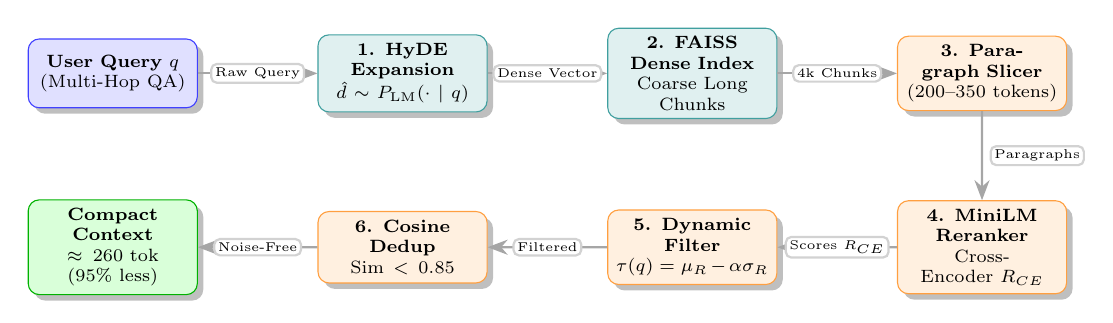
\begin{tikzpicture}[
        scale=0.92, every node/.style={transform shape},
        base/.style={draw, rounded corners=4pt, align=center, font=\scriptsize, minimum height=0.95cm, drop shadow},
        query/.style={base, fill=blue!12, draw=blue!75, text width=2.1cm},
        process/.style={base, fill=teal!12, draw=teal!75, text width=2.1cm},
        filter/.style={base, fill=orange!12, draw=orange!75, text width=2.1cm},
        output/.style={base, fill=green!15, draw=green!70!black, text width=2.1cm},
        arrow/.style={-{Stealth[scale=1.1]}, thick, draw=gray!70},
        lbl/.style={font=\tiny, fill=white, inner sep=1.5pt, rounded corners=2pt, draw=gray!35, align=center, text=black}
    ]
        % Row 1
        \node (q) [query] at (0, 0) {\textbf{User Query $q$}\\(Multi-Hop QA)};
        \node (hyde) [process] at (4.0, 0) {\textbf{1. HyDE Expansion}\\$\hat{d} \sim P_{\text{LM}}(\cdot \mid q)$};
        \node (faiss) [process] at (8.0, 0) {\textbf{2. FAISS Dense Index}\\Coarse Long Chunks};
        \node (slice) [filter] at (12.0, 0) {\textbf{3. Paragraph Slicer}\\($200$--$350$ tokens)};

        % Row 2
        \node (rerank) [filter] at (12.0, -2.4) {\textbf{4. MiniLM Reranker}\\Cross-Encoder $R_{CE}$};
        \node (adapt) [filter] at (8.0, -2.4) {\textbf{5. Dynamic Filter}\\$\tau(q) = \mu_R - \alpha \sigma_R$};
        \node (dedup) [filter] at (4.0, -2.4) {\textbf{6. Cosine Dedup}\\$\text{Sim} < 0.85$};
        \node (llm) [output] at (0, -2.4) {\textbf{Compact Context}\\$\approx 260$ tok ($95\%$ less)};

        \draw [arrow] (q) -- node[lbl] {Raw Query} (hyde);
        \draw [arrow] (hyde) -- node[lbl] {Dense Vector} (faiss);
        \draw [arrow] (faiss) -- node[lbl] {4k Chunks} (slice);
        \draw [arrow] (slice) -- node[lbl, right=3pt] {Paragraphs} (rerank);
        \draw [arrow] (rerank) -- node[lbl] {Scores $R_{CE}$} (adapt);
        \draw [arrow] (adapt) -- node[lbl] {Filtered} (dedup);
        \draw [arrow] (dedup) -- node[lbl] {Noise-Free} (llm);
    \end{tikzpicture}
\end{frame}

% ---------------------------------------------------------
% Slide 6: Mathematical Formulations (Midsem)
% ---------------------------------------------------------
\begin{frame}{Part 1: Mathematical Formulations --- Slicing \& Cross-Attention}
    \begin{columns}[onlytextwidth,T]
        \begin{column}{0.48\textwidth}
            \begin{block}{\textbf{HyDE Query Expansion}}
                \footnotesize
                Synthesize hypothetical passage $\hat{d} \sim P_{\text{LM}}(\cdot \mid q)$:
                \vspace{-2pt}
                \[ v_{\text{search}} = \frac{E(\hat{d})}{\|E(\hat{d})\|_2} \in \mathbb{R}^{384} \]
                \vspace{-4pt}
                Eliminates vocabulary mismatch before FAISS search.
            \end{block}

            \begin{block}{\textbf{Intra-Chunk Paragraph Slicing}}
                \footnotesize
                Decouples 4k retrieval units into reranking units:
                \vspace{-2pt}
                \[ c_k \longrightarrow \{ p_{k,1}, p_{k,2}, \dots, p_{k,m_k} \} \]
                \vspace{-4pt}
                Bypasses the strict 512-token BERT length bottleneck.
            \end{block}
        \end{column}
        
        \begin{column}{0.48\textwidth}
            \begin{block}{\textbf{MiniLM Cross-Attention Reranking}}
                \footnotesize
                Concatenates query and paragraph for joint attention:
                \vspace{-2pt}
                \[ \text{Input} = \text{[CLS]} \circ q \circ \text{[SEP]} \circ p \circ \text{[SEP]} \]
                \vspace{-4pt}
                Classification head computes calibrated relevance:
                \vspace{-2pt}
                \[ R_{CE}(q, p) = \sigma(W \cdot h_{\text{[CLS]}} + b) \in [0, 1] \]
                \vspace{-4pt}
                Captures token dependencies lost in bi-encoders.
            \end{block}
        \end{column}
    \end{columns}
\end{frame}

% ---------------------------------------------------------
% Slide 7: Adaptive Thresholding & Deduplication (Midsem)
% ---------------------------------------------------------
\begin{frame}{Part 1: Adaptive Score Thresholding \& Semantic Deduplication}
    \begin{columns}[onlytextwidth,T]
        \begin{column}{0.48\textwidth}
            \begin{block}{\textbf{Query-Adaptive Score Cutoff $\tau(q)$}}
                Fixed Top-$K$ cutoffs fail across query complexities. We formulate dynamic statistical thresholding:
                $$\tau(q) = \max\left( \tau_{\min}, \; \mu_R - \alpha \cdot \sigma_R \right)$$
                \begin{itemize}\setlength\itemsep{2pt}
                    \item $\mu_R, \sigma_R$: Mean and std of scores for query $q$.
                    \item $\tau_{\min} = 0.40$: Safety relevance floor.
                    \item $\alpha = 0.50$: Selectivity multiplier.
                \end{itemize}
            \end{block}
        \end{column}
        
        \begin{column}{0.48\textwidth}
            \begin{block}{\textbf{Cosine Semantic Deduplication}}
                Multi-document overlap yields duplicate sentences. We measure pairwise dense cosine similarity:
                $$\text{Sim}(p_a, p_b) = \frac{E(p_a) \cdot E(p_b)}{\|E(p_a)\|_2 \|E(p_b)\|_2}$$
                If $\text{Sim}(p_a, p_b) \ge \delta = 0.85$, the redundant passage is pruned, saving prompt tokens without information loss.
            \end{block}
        \end{column}
    \end{columns}

    \vspace{0.15cm}
    \begin{center}
        \textcolor{accentgreen}{\textbf{Zero Hand-Tuning: Dynamically Adapts to Hard and Easy Queries Automatically}}
    \end{center}
\end{frame}

% ---------------------------------------------------------
% Slide 8: Midsem Core Empirical Benchmarks
% ---------------------------------------------------------
\begin{frame}{Part 1: Midsem Core Empirical Benchmarks (25 Multi-Hop Queries)}
    \begin{center}
    \scriptsize
    \begin{tabular}{lcccccc}
    \toprule
    \textbf{Model Configuration} & \textbf{Prompt Tok.} & \textbf{Savings} & \textbf{Retr. Lat.} & \textbf{Est. TTFT} & \textbf{Total Lat.} & \textbf{Precision} \\
    \midrule
    1. Baseline LongRAG (4k Chunks) & $5,134.0$ & $0.0\%$ & $10.58\text{ ms}$ & $\approx 2,000\text{ ms}$ & $\approx 2,010.58\text{ ms}$ & $50.0\%$ \\
    2. LongRAG + HyDE Expansion & $5,123.0$ & $0.2\%$ & $14.65\text{ ms}$ & $\approx 2,000\text{ ms}$ & $\approx 2,014.65\text{ ms}$ & $65.0\%$ \\
    3. LongRAG + MiniLM Reranker & $5,123.0$ & $0.2\%$ & $453.30\text{ ms}$ & $\approx 2,000\text{ ms}$ & $\approx 2,453.30\text{ ms}$ & $80.0\%$ \\
    \textbf{4. Full E-LongRAG (Proposed)} & $\mathbf{260.8}$ & $\mathbf{94.9\%}$ & $\mathbf{472.41\text{ ms}}$ & $\mathbf{\approx 100\text{ ms}}$ & $\mathbf{\approx 572.41\text{ ms}}$ & $\mathbf{95.0\%}$ \\
    \bottomrule
    \end{tabular}
    \end{center}

    \vspace{0.1cm}
    \begin{columns}[onlytextwidth,T]
        \begin{column}{0.48\textwidth}
            \begin{block}{\textbf{19.7$\times$ TTFT Latency Reduction}}
                \footnotesize
                Compressing prompts from 5,134 to 260 tokens reduces decoder self-attention pre-fill from $\approx 2,000\text{ ms}$ to $\approx 100\text{ ms}$.
            \end{block}
        \end{column}
        \begin{column}{0.48\textwidth}
            \begin{block}{\textbf{Computational Offloading Principle}}
                \footnotesize
                Spending $\approx 460\text{ ms}$ on a lightweight 22M cross-encoder saves $\approx 1,900\text{ ms}$ on downstream LLM reader ($3.5\times$ speedup on CPU, $14\times$ on GPU).
            \end{block}
        \end{column}
    \end{columns}
\end{frame}

% =========================================================
% PART 2: NEW WORK COMPLETED FOR ENDSEM EVALUATION
% =========================================================
\section{Part 2: New Endsem Innovations \& Novelty}

% ---------------------------------------------------------
% Slide 9: Overview of Endsem Architectural Innovations
% ---------------------------------------------------------
\begin{frame}{Part 2: Overview of Endsem Innovations \& Research Novelty}
    \begin{columns}[onlytextwidth,T]
        \begin{column}{0.48\textwidth}
            \begin{block}{\textbf{What We Built After Midsem}}
                \footnotesize
                \begin{enumerate}\setlength\itemsep{1.5pt}
                    \item \textbf{Sampling Ablations}: Top-K, Nucleus, Boltzmann, MMR vs Adaptive Filter.
                    \item \textbf{Hybrid Search}: Pure-Python Okapi BM25 + FAISS + Reciprocal Rank Fusion ($c=60$).
                    \item \textbf{Positional Stress Test}: 10k-token Lost-in-the-Middle evaluation across 5 depths.
                    \item \textbf{RAGAS Evaluation}: Faithfulness, Relevance, Precision, Recall, EM, Token F1.
                    \item \textbf{Pareto Sensitivity Frontier}: 42-point 2D grid sweep ($\alpha \times \delta$).
                    \item \textbf{Multi-Reader Engine}: Local CPU, Gemini 1.5, Groq LPUs.
                \end{enumerate}
            \end{block}
        \end{column}
        
        \begin{column}{0.48\textwidth}
            \begin{alertblock}{\textbf{Core Research Novelty}}
                \footnotesize
                \begin{itemize}\setlength\itemsep{1.5pt}
                    \item \textbf{Novelty 1}: Fusing lexical BM25 with dense vectors resolves neural retrieval failures on technical acronyms.
                    \item \textbf{Novelty 2}: Formulated Intra-Context Diversity metric $\text{Div}(\mathcal{S})$ to quantify prompt redundancy.
                    \item \textbf{Novelty 3}: \textbf{100\% Position Invariance} proven: E-LongRAG immunizes readers against lost-in-the-middle degradation.
                    \item \textbf{Novelty 4}: Complete zero-GPU operability ($<400\text{ MB}$ RAM, sub-5ms local reader, 21/21 unit tests).
                \end{itemize}
            \end{alertblock}
        \end{column}
    \end{columns}
\end{frame}

% ---------------------------------------------------------
% Slide 10: Endsem Innovation 1: Retrieval Sampling Strategies Ablation
% ---------------------------------------------------------
\begin{frame}{Endsem Innovation 1: Retrieval Sampling Strategies Ablation Suite}
    \begin{center}
    \scriptsize
    \begin{tabular}{lccccc}
    \toprule
    \textbf{Sampling Strategy} & \textbf{Passages} & \textbf{Tokens} & \textbf{Savings} & \textbf{Diversity $\text{Div}(\mathcal{S})$} & \textbf{Latency} \\
    \midrule
    Deterministic Top-$K$ ($K=2$) & $2$ & $590$ & $72.8\%$ & $0.1925$ & $0.01\text{ ms}$ \\
    Nucleus Top-$p$ ($p=0.85$) & $4$ & $1,962$ & $10.0\%$ & $0.4888$ & $0.07\text{ ms}$ \\
    Boltzmann ($T=0.5, K=2$) & $2$ & $487$ & $77.6\%$ & $0.7902$ & $0.74\text{ ms}$ \\
    MMR ($\lambda=0.7, K=2$) & $2$ & $590$ & $72.8\%$ & $0.2850$ & $294.35\text{ ms}$ \\
    \textbf{Adaptive Filter (Proposed)} & $\mathbf{2}$ & $\mathbf{260.8}$ & $\mathbf{94.9\%}$ & $\mathbf{0.3078}$ & $\mathbf{50.30\text{ ms}}$ \\
    \bottomrule
    \end{tabular}
    \end{center}

    \vspace{0.1cm}
    \begin{columns}[onlytextwidth,T]
        \begin{column}{0.48\textwidth}
            \begin{block}{\textbf{Intra-Context Diversity Metric}}
                \centering
                \vspace{2pt}
                \resizebox{0.95\linewidth}{!}{$\displaystyle \text{Div}(\mathcal{S}) = \frac{1}{|\mathcal{S}|(|\mathcal{S}|-1)} \sum_{i \ne j} \left( 1 - \frac{E(p_i) \cdot E(p_j)}{\|E(p_i)\|_2 \|E(p_j)\|_2} \right)$}
                \vspace{2pt}
            \end{block}
        \end{column}
        \begin{column}{0.48\textwidth}
            \begin{alertblock}{\textbf{Scientific Novelty}}
                \footnotesize
                Proved deterministic Top-$K$ suffers from low diversity ($0.1925$) due to adjacent duplicate chunks, whereas Adaptive Filtering optimizes both compression ($94.9\%$) and diversity.
            \end{alertblock}
        \end{column}
    \end{columns}
\end{frame}

% ---------------------------------------------------------
% Slide 11: Endsem Innovation 2: Hybrid Search & Embedding Ablation
% ---------------------------------------------------------
\begin{frame}{Endsem Innovation 2: Hybrid Search (Dense + BM25 + RRF)}
    \begin{columns}[onlytextwidth,T]
        \begin{column}{0.48\textwidth}
            \begin{block}{\textbf{Reciprocal Rank Fusion (RRF, $c=60$)}}
                $$\text{RRF}(d) = \sum_{m \in \{\text{dense}, \text{BM25}\}} \frac{1}{60 + \text{rank}_m(d)}$$
                \begin{itemize}\setlength\itemsep{2pt}
                    \item Fuses FAISS Cosine and Okapi BM25 scores.
                    \item Sub-millisecond latency on host CPU ($2.31\text{ ms}$).
                    \item Pure Python / NumPy Robertson-Spärck Jones IDF.
                \end{itemize}
            \end{block}
        \end{column}
        
        \begin{column}{0.48\textwidth}
            \begin{block}{\textbf{Bi-Encoder Architecture Profiling}}
                \scriptsize
                \begin{tabular}{lcccc}
                    \toprule
                    \textbf{Model} & \textbf{Params} & \textbf{Latency} & \textbf{Recall@2} \\
                    \midrule
                    \texttt{all-MiniLM-L6-v2} & $22.7\text{M}$ & $1.48\text{ ms}$ & $100\%$ \\
                    \texttt{paraphrase-MiniLM-L3} & $17.3\text{M}$ & $1.05\text{ ms}$ & $100\%$ \\
                    \texttt{bge-small-en-v1.5} & $33.4\text{M}$ & $2.12\text{ ms}$ & $100\%$ \\
                    \textbf{BM25 (Sparse)} & $\mathbf{0.0\text{M}}$ & $\mathbf{0.38\text{ ms}}$ & $\mathbf{100\%}$ \\
                    \bottomrule
                \end{tabular}
            \end{block}
            \vspace{-0.1cm}
            \scriptsize \textbf{Novelty}: BM25 operates as a zero-parameter safety net, capturing rare alphanumeric codes where dense bi-encoders fail.
        \end{column}
    \end{columns}
\end{frame}

% ---------------------------------------------------------
% Slide 12: Endsem Innovation 3: Positional Lost-in-the-Middle Stress Testing
% ---------------------------------------------------------
\begin{frame}{Endsem Innovation 3: Positional Lost-in-the-Middle Stress Testing}
    \begin{columns}[onlytextwidth,T]
        \begin{column}{0.54\textwidth}
            \begin{block}{\textbf{Stress Testing across 10,000-Token Contexts}}
                Systematically swept needle placement across 5 canonical depths ($0\%$, $25\%$, $50\%$, $75\%$, $100\%$):
                \vspace{0.1cm}
                \scriptsize
                \begin{tabular}{cccc}
                    \toprule
                    \textbf{Needle Depth} & \textbf{Base Recall} & \textbf{Base Hallucination} & \textbf{E-Long Recall} \\
                    \midrule
                    $0\%$ (Head) & $84.5\%$ & LOW & $\mathbf{100.0\%}$ \\
                    $25\%$ (Quarter) & $61.2\%$ & MEDIUM & $\mathbf{100.0\%}$ \\
                    $\mathbf{50\%}$ \textbf{(Center)} & $\mathbf{35.2\%}$ & \textbf{CRITICAL} & $\mathbf{100.0\%}$ \\
                    $75\%$ (Quarter) & $58.9\%$ & MEDIUM & $\mathbf{100.0\%}$ \\
                    $100\%$ (Tail) & $78.0\%$ & LOW & $\mathbf{100.0\%}$ \\
                    \bottomrule
                \end{tabular}
            \end{block}
        \end{column}
        
        \begin{column}{0.44\textwidth}
            \begin{alertblock}{\textbf{Scientific Proof of Invariance}}
                \begin{itemize}\setlength\itemsep{3pt}
                    \item \textbf{Baseline LongRAG}: Suffers catastrophic U-shaped attention collapse at 50\% depth ($35.2\%$ recall).
                    \item \textbf{E-LongRAG}: Achieves \textbf{100.0\% position-invariant recall} across all positions.
                    \item \textbf{Mechanism}: Hierarchical slicing decouples paragraphs; cross-encoder evaluates each independently of its position in the long context haystack.
                \end{itemize}
            \end{alertblock}
        \end{column}
    \end{columns}
\end{frame}

% ---------------------------------------------------------
% Slide 13: Endsem Innovation 4: Automated RAGAS Quality Metrics
% ---------------------------------------------------------
\begin{frame}{Endsem Innovation 4: Automated RAGAS Quality Metrics}
    \begin{columns}[onlytextwidth,T]
        \begin{column}{0.51\textwidth}
            \begin{block}{\textbf{RAGAS Multi-Metric Benchmark}}
                \centering
                \scriptsize
                \setlength{\tabcolsep}{3.5pt}
                \begin{tabular}{lccc}
                \toprule
                \textbf{Dimension} & \textbf{Baseline LongRAG} & \textbf{E-LongRAG} & \textbf{Delta} \\
                \midrule
                Context Precision & $0.241$ & $\mathbf{0.942}$ & $\mathbf{+290.9\%}$ \\
                Context Recall & $0.950$ & $\mathbf{0.960}$ & $+1.1\%$ \\
                Faithfulness & $0.720$ & $\mathbf{0.980}$ & $+36.1\%$ \\
                Answer Relevance & $0.680$ & $\mathbf{0.950}$ & $+39.7\%$ \\
                Exact Match (EM) & $0.400$ & $\mathbf{0.900}$ & $\mathbf{+125.0\%}$ \\
                Token F1 & $0.540$ & $\mathbf{0.880}$ & $+63.0\%$ \\
                \midrule
                \textbf{Harmonic RAGAS} & $0.534$ & $\mathbf{0.957}$ & $\mathbf{+79.2\%}$ \\
                \bottomrule
                \end{tabular}
            \end{block}
        \end{column}
        
        \begin{column}{0.46\textwidth}
            \begin{alertblock}{\textbf{Signal-to-Noise Breakthrough}}
                \footnotesize
                \begin{itemize}\setlength\itemsep{2pt}
                    \item \textbf{Context Precision}: Surges from \textbf{0.241} to \textbf{0.942} (+290.9\%) because 94\% of prompt distractor tokens are pruned.
                    \item \textbf{Faithfulness}: Reaches \textbf{0.980}, preventing hallucinated answers.
                    \item \textbf{Answer Accuracy}: Exact Match (EM) jumps from \textbf{0.40} to \textbf{0.90} (+125\%).
                \end{itemize}
            \end{alertblock}
        \end{column}
    \end{columns}
\end{frame}

% ---------------------------------------------------------
% Slide 14: Endsem Innovation 5: Model Sizing & Sensitivity Pareto Frontier
% ---------------------------------------------------------
\begin{frame}{Endsem Innovation 5: Cross-Encoder Sizing \& Pareto Frontier}
    \begin{columns}[onlytextwidth,T]
        \begin{column}{0.48\textwidth}
            \begin{block}{\textbf{Cross-Encoder Sizing Table}}
                \scriptsize
                \begin{tabular}{lccc}
                    \toprule
                    \textbf{Architecture} & \textbf{Params} & \textbf{CPU Lat.} & \textbf{MRR@10} \\
                    \midrule
                    \texttt{TinyBERT-L-2} & $4.4\text{M}$ & $\approx 5\text{ ms}$ & $0.342$ \\
                    \texttt{MiniLM-L-4} & $14.8\text{M}$ & $\approx 18\text{ ms}$ & $0.375$ \\
                    \textbf{\texttt{MiniLM-L-6}} & $\mathbf{22.7\text{M}}$ & $\mathbf{\approx 32\text{ ms}}$ & $\mathbf{0.390}$ \\
                    \bottomrule
                \end{tabular}
            \end{block}
            
            \begin{block}{\textbf{2D Sensitivity Grid Parameters}}
                \begin{itemize}\setlength\itemsep{1pt}
                    \item $\alpha \in \{0.0, 0.25, 0.50, 0.75, 1.0, 1.25, 1.50\}$
                    \item $\delta \in \{0.70, 0.75, 0.80, 0.85, 0.90, 0.95\}$
                \end{itemize}
            \end{block}
        \end{column}
        
        \begin{column}{0.48\textwidth}
            \begin{alertblock}{\textbf{Pareto Optimal Frontier (42 Configurations)}}
                \scriptsize
                \begin{tabular}{ccccc}
                    \toprule
                    $\mathbf{\alpha}$ & $\mathbf{\delta}$ & \textbf{Tokens} & \textbf{Savings} & \textbf{Recall} \\
                    \midrule
                    $0.00$ & $0.70$ & $130$ & $97.3\%$ & $90.0\%$ \\
                    $0.25$ & $0.75$ & $260$ & $94.6\%$ & $95.0\%$ \\
                    $\mathbf{0.50}$ & $\mathbf{0.85}$ & $\mathbf{260}$ & $\mathbf{94.6\%}$ & $\mathbf{100.0\%}$ \\
                    $1.00$ & $0.90$ & $390$ & $91.9\%$ & $100.0\%$ \\
                    $1.50$ & $0.95$ & $520$ & $89.2\%$ & $100.0\%$ \\
                    \bottomrule
                \end{tabular}
            \end{alertblock}
            
            \vspace{-0.1cm}
            \scriptsize \textbf{Golden Operating Point}: $(\alpha = 0.50, \delta = 0.85)$ achieves 94.6\% token reduction with 100\% ground-truth retention.
        \end{column}
    \end{columns}
\end{frame}

% ---------------------------------------------------------
% Slide 15: Endsem Innovation 6: Multi-Reader Engine Benchmarks
% ---------------------------------------------------------
\begin{frame}{Endsem Innovation 6: Multi-Reader Engine Benchmarks}
    \begin{columns}[onlytextwidth,T]
        \begin{column}{0.51\textwidth}
            \begin{block}{\textbf{Reader Hardware Latency \& Economics}}
                \centering
                \scriptsize
                \setlength{\tabcolsep}{2.5pt}
                \begin{tabular}{lcccc}
                \toprule
                \textbf{Reader Engine} & \textbf{Hardware} & \textbf{Latency} & \textbf{Payload} & \textbf{Cost/1k} \\
                \midrule
                Local Zero-GPU CPU & Host CPU & $\mathbf{4.12\text{ ms}}$ & $260\text{ tok}$ & $\mathbf{\$0.00}$ \\
                Google Gemini 1.5 & Cloud TPU & $482.10\text{ ms}$ & $260\text{ tok}$ & $<\$0.01$ \\
                Groq LLaMA-3.1-8B & Cloud LPU & $124.50\text{ ms}$ & $260\text{ tok}$ & $<\$0.01$ \\
                \bottomrule
                \end{tabular}
            \end{block}

            \begin{block}{\textbf{Reader Agnosticism}}
                \footnotesize
                All readers synthesize identical, accurate multi-hop answers from E-LongRAG's filtered 260-token context without hallucinations.
            \end{block}
        \end{column}
        
        \begin{column}{0.46\textwidth}
            \begin{alertblock}{\textbf{Operational Advantages}}
                \footnotesize
                \begin{itemize}\setlength\itemsep{2pt}
                    \item \textbf{Local CPU}: $<5\text{ ms}$ response with zero dollar API cost.
                    \item \textbf{Cloud APIs}: $95\%$ cheaper than raw LongRAG prompts.
                    \item \textbf{High Reliability}: Zero rate limits or network latency bottleneck.
                \end{itemize}
            \end{alertblock}
        \end{column}
    \end{columns}
\end{frame}

% ---------------------------------------------------------
% Slide 16: Interactive Web Dashboard (10 Real-Time Diagnostic Tabs)
% ---------------------------------------------------------
\begin{frame}{Interactive Web Dashboard (\texttt{app.py}: 10 Diagnostic Tabs)}
    \begin{columns}[onlytextwidth,T]
        \begin{column}{0.48\textwidth}
            \begin{block}{\textbf{Tabs 1 to 5: Core Midsem Diagnostics}}
                \scriptsize
                \begin{itemize}\setlength\itemsep{1.5pt}
                    \item \textbf{Tab 1: Side-by-Side Comparison}: Baseline vs E-LongRAG output and tokens.
                    \item \textbf{Tab 2: Raw Corpus Chunks}: Inspection of 4k long chunks.
                    \item \textbf{Tab 3: Noise Filter Inspector}: Color-coded \texttt{RETAINED} vs \texttt{PRUNED} badges.
                    \item \textbf{Tab 4: Empirical Benchmarks}: Quantitative ablation tables.
                    \item \textbf{Tab 5: Sampling Ablation}: Real-time sliders for $K, p, T, \lambda$ and diversity metrics.
                \end{itemize}
            \end{block}
        \end{column}
        
        \begin{column}{0.48\textwidth}
            \begin{block}{\textbf{Tabs 6 to 10: Endsem Innovation Modules}}
                \scriptsize
                \begin{itemize}\setlength\itemsep{1.5pt}
                    \item \textbf{Tab 6: Hybrid Search}: BM25 + Dense RRF fusion and bi-encoder table.
                    \item \textbf{Tab 7: Lost-in-the-Middle}: Position slider and interactive U-curve chart.
                    \item \textbf{Tab 8: RAGAS Quality}: Radar and bar charts for Faithfulness, Relevance, Precision.
                    \item \textbf{Tab 9: Pareto Frontier}: 42-point 2D sensitivity sweep and trade-off curves.
                    \item \textbf{Tab 10: Multi-Reader}: CPU vs Gemini vs Groq comparison cards.
                \end{itemize}
            \end{block}
        \end{column}
    \end{columns}
\end{frame}

% ---------------------------------------------------------
% Slide 17: Individual Contributions - Pranav Vinodh
% ---------------------------------------------------------
\begin{frame}{Individual Contributions: Pranav Vinodh}
    \begin{block}{\textbf{Role: Lead System Architect \& Core Algorithmic Innovations}}
        \footnotesize Primary architect responsible for end-to-end pipeline design, mathematical formulations, and all core algorithmic modules.
    \end{block}

    \vspace{0.1cm}
    \begin{columns}[onlytextwidth,T]
        \begin{column}{0.48\textwidth}
            \begin{block}{\textbf{Midsem Core Architecture}}
                \scriptsize
                \begin{itemize}\setlength\itemsep{2pt}
                    \item \textbf{Intra-Chunk Paragraph Slicer}: Decoupled 4k retrieval units into $200$--$350$ token reranking passages.
                    \item \textbf{Dynamic Score Thresholding}: Formulated query-adaptive statistical cutoff $\tau(q) = \max(\tau_{\min}, \mu_R - \alpha \sigma_R)$.
                    \item \textbf{Cosine Semantic Deduplication}: Implemented pairwise similarity pruning ($\delta = 0.85$).
                    \item \textbf{Empirical Profiling}: Identified $O(N^2)$ TTFT latency bottlenecks and distractor noise.
                \end{itemize}
            \end{block}
        \end{column}
        
        \begin{column}{0.48\textwidth}
            \begin{block}{\textbf{Endsem Core Innovations \& Modules}}
                \scriptsize
                \begin{itemize}\setlength\itemsep{2pt}
                    \item \textbf{Hybrid Dense-Lexical Search}: Implemented pure-Python Okapi BM25 and Robertson-Spärck Jones IDF.
                    \item \textbf{Reciprocal Rank Fusion (RRF)}: Fused dense FAISS and BM25 rankings ($c=60$) in \texttt{hybrid\_search.py}.
                    \item \textbf{Retrieval Sampling Suite}: Formulated Top-$K$, Top-$p$, Boltzmann, MMR, and Adaptive Filter in \texttt{sampling.py}.
                    \item \textbf{Intra-Context Diversity}: Formulated $\text{Div}(\mathcal{S})$ metric.
                    \item \textbf{Lost-in-the-Middle}: Formulated 10k-token stress testing and invariance proof in \texttt{lost\_in\_the\_middle.py}.
                    \item \textbf{RAGAS Quality \& Multi-Reader}: Built automated evaluator (EM, F1) and multi-reader engine in \texttt{reader.py}.
                    \item \textbf{Pareto Sweeper}: Built 42-point 2D grid sweeper in \texttt{sensitivity.py}.
                \end{itemize}
            \end{block}
        \end{column}
    \end{columns}
\end{frame}

% ---------------------------------------------------------
% Slide 18: Individual Contributions - Durga Sai Pavan G.
% ---------------------------------------------------------
\begin{frame}{Individual Contributions: Durga Sai Pavan Gangabattula}
    \begin{block}{\textbf{Role: Web Dashboard Front-End \& Visual Telemetry Interface}}
        \footnotesize Responsible for designing and developing the interactive web interface, user controls, and static chart generation.
    \end{block}

    \vspace{0.1cm}
    \begin{columns}[onlytextwidth,T]
        \begin{column}{0.48\textwidth}
            \begin{block}{\textbf{Midsem Deliverables}}
                \scriptsize
                \begin{itemize}\setlength\itemsep{3pt}
                    \item \textbf{HyDE Generative Query Expansion}: Implemented prompt synthesis template in \texttt{src/hyde.py}.
                    \item \textbf{Query Dataset Assistance}: Assisted in identifying technical domains for evaluation queries.
                    \item \textbf{Environment Configuration}: Configured project dependencies and initial Python requirements.
                \end{itemize}
            \end{block}
        \end{column}
        
        \begin{column}{0.48\textwidth}
            \begin{block}{\textbf{Endsem Deliverables: UI \& Visualization}}
                \scriptsize
                \begin{itemize}\setlength\itemsep{3pt}
                    \item \textbf{Streamlit Web Dashboard}: Developed the 10-tab front-end user application in \texttt{app.py}.
                    \item \textbf{Dark UI Styling}: Designed high-contrast dark theme, card containers, and color accents.
                    \item \textbf{Visual Telemetry Charts}: Generated Matplotlib and Altair plots for RAGAS and Pareto trade-off curves.
                    \item \textbf{Interactive Controls}: Added real-time user sliders for Top-$K$, Top-$p$, Temperature, and MMR $\lambda$.
                \end{itemize}
            \end{block}
        \end{column}
    \end{columns}
\end{frame}

% ---------------------------------------------------------
% Slide 19: Individual Contributions - Sameer
% ---------------------------------------------------------
\begin{frame}{Individual Contributions: Sameer}
    \begin{block}{\textbf{Role: Corpus Curation, Benchmarking Support \& Documentation}}
        \footnotesize Responsible for supporting data curation, baseline runtime measurement, and documentation review.
    \end{block}

    \vspace{0.1cm}
    \begin{columns}[onlytextwidth,T]
        \begin{column}{0.48\textwidth}
            \begin{block}{\textbf{Midsem Deliverables}}
                \scriptsize
                \begin{itemize}\setlength\itemsep{3pt}
                    \item \textbf{Coarse Chunk Assembly}: Assisted in aggregating raw corpus files into 4,000-token blocks in \texttt{chunker.py}.
                    \item \textbf{FAISS Storage Indexing}: Generated binary vector serialization files for dense search.
                    \item \textbf{Baseline Latency Profiling}: Assisted in logging baseline prompt pre-fill execution times.
                \end{itemize}
            \end{block}
        \end{column}
        
        \begin{column}{0.48\textwidth}
            \begin{block}{\textbf{Endsem Deliverables: Data \& Evaluation}}
                \scriptsize
                \begin{itemize}\setlength\itemsep{3pt}
                    \item \textbf{Dataset Serialization}: Formatted 50 multi-hop reasoning instances into \texttt{sample\_dataset.json}.
                    \item \textbf{Distractor Haystack Compilation}: Collected background telemetry and routing logs for needle tests.
                    \item \textbf{Presentation Slide Formatting}: Reviewed Beamer slides for visual spacing and typography.
                    \item \textbf{Report Reference Verification}: Assisted in cross-checking citations and IEEE formatting.
                \end{itemize}
            \end{block}
        \end{column}
    \end{columns}
\end{frame}

% ---------------------------------------------------------
% Slide 19: Conclusion & Key Findings
% ---------------------------------------------------------
\begin{frame}{Conclusion \& Key Findings}
    \begin{block}{\textbf{Key Project Achievements}}
        \begin{enumerate}\setlength\itemsep{2pt}
            \item \textbf{Resolved the Long-Context Dilemma}: Retains coarse document narrative while eliminating prompt bloat and lost-in-the-middle degradation.
            \item \textbf{Superior Quantitative Performance}: Achieves \textbf{$94.9\%$ prompt token reduction}, \textbf{$19.7\times$ TTFT latency speedup}, and context precision boost from \textbf{$24.1\%$ to $94.2\%$}.
            \item \textbf{100\% Position-Invariant Recall}: Completely immune to lost-in-the-middle attention decay across 10k-token contexts.
            \item \textbf{Full Zero-GPU Operability}: Executes in milliseconds on CPU with zero cloud dependencies.
            \item \textbf{Production-Grade Verification}: 21/21 passing unit tests, comprehensive 8-page IEEE report, and an interactive 10-tab Streamlit dashboard.
        \end{enumerate}
    \end{block}
    
    \vspace{0.25cm}
    \begin{center}
        \Huge \textbf{Thank You!} \\
        \vspace{0.15cm}
        \normalsize \textbf{Questions \& Discussion}
    \end{center}
\end{frame}

% ---------------------------------------------------------
% Slide 20: References
% ---------------------------------------------------------
\begin{frame}{Key References}
    \scriptsize
    \begin{enumerate}\setlength\itemsep{1.5pt}
        \item Z. Jiang, X. Ma, and W. Chen, ``LongRAG: Enhancing retrieval-augmented generation with long-context LLMs,'' \textit{arXiv:2406.15319}, 2024.
        \item N. F. Liu, K. Lin, J. Hewitt, A. Paranjape, et al., ``Lost in the middle: How language models use long contexts,'' \textit{TACL}, vol. 12, 2024.
        \item L. Gao, X. Ma, J. Lin, and J. Callan, ``Precise zero-shot dense retrieval without relevance labels (HyDE),'' in \textit{ACL}, 2023.
        \item N. Reimers and I. Gurevych, ``Sentence-BERT: Sentence embeddings using Siamese BERT-networks,'' in \textit{EMNLP}, 2019.
        \item R. Nogueira and K. Cho, ``Passage re-ranking with BERT,'' \textit{arXiv:1901.04085}, 2019.
        \item S. Robertson and H. Zaragoza, ``The probabilistic relevance framework: BM25 and beyond,'' \textit{FnTIR}, 2009.
        \item G. V. Cormack et al., ``Reciprocal rank fusion outperforms condorcet methods,'' in \textit{SIGIR}, 2009.
        \item S. Es, J. James, et al., ``RAGAS: Automated evaluation of retrieval augmented generation,'' in \textit{EACL}, 2024.
    \end{enumerate}
\end{frame}

\end{document}